%!TEX root = ../Security&NetworkManagement.tex
\appendix
\chapter{Penetration Test}
Di seguito vengono illutrati alcuni appunti riguardanti lezioni e seminari sul penetration testing.\\

Il Penetration Test è il processo operativo di valutazione della sicurezza di un sistema o di una rete che simula l'attacco di un utente malintenzionato. L'analisi comprende più fasi ed ha come obiettivo evidenziare le debolezze della piattaforma fornendo il maggior numero di informazioni sulle vulnerabilità che ne hanno permesso l'accesso non autorizzato. Perchè si esegue?
\begin{itemize}
\item Per scoprire bug nel software
\item Per scoprire se i sistemi sono mal configurati (es. Firewall con porte aperte)
\item Per valutare la bontà dell'infrastruttura e proporre un upgrade
\item Per sfruttare i buchi identificati per far vedere che è possibile accedere al sistema e ai dati
\end{itemize}

L'analisi è condotta dal punto di vista di un potenziale attaccante e consiste nello sfruttamento delle vulnerabilità rilevate al fine di ottenere più informazioni possibili per accedere indebitamente al sistema. Un penetration test può aiutare a determinare se le difese del sistema sono sufficienti o se presenta delle vulnerabilità elencando in questo caso quali difese il test ha sconfitto. 

Il sistema può avere diversi livelli e tipi di vulnerabilità: interne, esterne o sicurezza fisica. si parla quindi di outside pentest (si esegue tramite collagamento internet e lavora a livello 3 dello stack TCP/IP) e inside pentest (accesso fisico alla rete del cliente e lavora a livello 2 MAC).  L'analisi viene svolta a fronte di un accordo commerciale/tecnico. Chi svolge questa attività è chiamato penetration tester o auditor o con il più moderno ethical hacker (\textit{white hat} hacker). Si distingue dal \textit{black hat} hacker che usa i dati recuperati dal penetration testing per guardagnarci/usarli in modo malevolo e il \textit{grey hat} hacker (misto tra white e black). Esiste anche un'altra categoria chiamata \textit{script kiddie} che rappresenta quello che utilizzano tool di pentest senza sapere cosa fanno.

I processi di penetration test possono essere effettuati in diverse modalità. La differenza consiste sulla quantità e qualità delle informazioni disponibili ai pentester riguardo ai sistemi analizzati. I test Black Box non presuppongono precedente conoscenza dell'infrastruttura oggetto di analisi e gli esaminatori necessitano di determinare architettura e servizi dei sistemi prima di iniziare l'analisi. Nei test White Box sono invece fornite conoscenze dettagliate dell'infrastruttura da esaminare (spesso insieme agli schemi di rete), codice sorgente delle applicazioni e liste di indirizzi IP presenti nella rete. Esistono anche approcci misti definiti Grey Box.

\subsubsection{Metodologia di un Pentester}
La prima cosa da pensare è pensare come un attaccante reale. Non bisogna mai, però, oltrepassare il limite di comportamento etico e bisogna porre sempre massima attenzione ai dettagli e alle informazioni collezionate durante tutta la fase di testing. Inoltre un pentester si limita a dimostrare la capacità di ottenere accesso al sistema e ai dati.  L'aspetto legale ha un ruolo importante. Un pentester ha ricevuto un'autorizzazione (lettera di incarico) dal proprietario del sistema ad eseguire le operazioni e deve tracciare qualsiasi operazione effettuata con i suoi tool a disposizione (sicuri e provati). Il pentester deve definire quando verranno effettuate le operazioni, concordare con il cliente la catena di comunicazione, identificare il range di indirizzi dei sistemi in scope del pentest,  indicare possibili cause che possano bloccare la prosecuzione delle attività (es. indirizzo bloccato su firewall, congestione/blocco traffico di rete, problema grave su sistema esposto che deve essere subito
notificato). Non deve ovviamente divulgare qualsiasi informazione ottenuta durante il testing. 

\subsubsection{Fasi di un Penetration Test}
Esistono vari Framework che definiscono metodi e manuali per la realizzazione di un pentesting. Alcuni esempi sono OWASP, OSSTM e ISSAF. Di seguito sono elencate le varie fasi di un pentest come è illutrato anche dalla Figura \ref{img:pentest_phases}:
\begin{enumerate}
\item Ricognizione (footprinting o reconnaissance): Idea del \textquotedblleft Guardare ma non toccare". Si collezionano più informazioni possibili.
\item Scansione ed enumerazione vulnerabilità: Port scanner e mapping, enumerazione dei servizi, vulnerability assessment.
\item Sfruttamento delle vulnerabilità e tentativo di accesso ai sistemi: Recupero di password per accedere ai dati, Metasploit di database e programmi.
\item Collezionamento dati
\item Rimozione delle tracce
\item Stesura del report
\end{enumerate}
\begin{figure}[htbp]
	\centering
	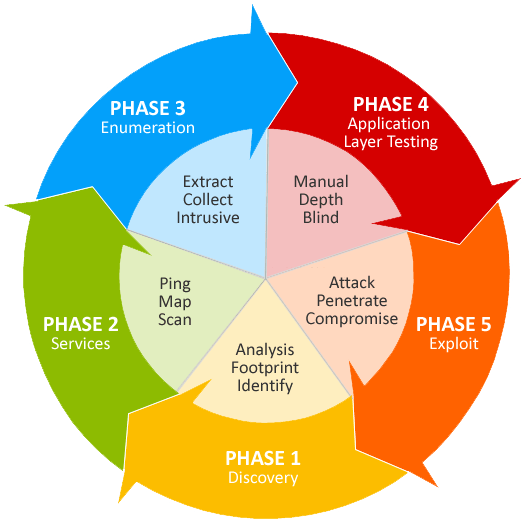
\includegraphics[scale = 0.4]{images/pentest_phases}
	\caption{Fasi di un Penetration Testing}
	\label{img:pentest_phases}
\end{figure}

\subsubsection{Distro linux per il Penetration Test}
\begin{itemize}
\item Kali linux
\item Backbox
\item Samurai web testing framework
\item Parrot Security
\item Caine (specializzata per analisi forense)
\item Deft (specializzata per analisi forense)
\end{itemize}